% Query Dual Dynamics Delta 中文翻译稿，仅供作者阅读和校对
\documentclass[11pt,a4paper]{ctexart}

\usepackage[left=2.35cm,right=2.35cm,top=2.4cm,bottom=2.4cm]{geometry}
\usepackage{graphicx}
\usepackage{amsmath,amssymb,amsfonts,amsthm,bm}
\usepackage{booktabs}
\usepackage{array}
\usepackage[numbers,sort&compress]{natbib}
\usepackage{xurl}
\usepackage[colorlinks=true,allcolors=blue]{hyperref}

\setmainfont{Times New Roman}
\setCJKmainfont[AutoFakeBold=2,AutoFakeSlant=0.2]{Noto Serif SC}
\setCJKsansfont{Microsoft YaHei}
\linespread{1.12}
\setlength{\parindent}{2em}
\setlength{\parskip}{0.15em}
\setlength{\emergencystretch}{2em}

\newtheorem{proposition}{命题}
\renewcommand{\proofname}{证明}
\renewcommand{\figurename}{图}
\renewcommand{\tablename}{表}

\newcommand{\R}{\mathbb{R}}
\newcommand{\M}{\bm{M}}
\newcommand{\Q}{\bm{Q}}
\newcommand{\U}{\bm{U}}
\newcommand{\kvec}{\bm{k}}
\newcommand{\qvec}{\bm{q}}
\newcommand{\vvec}{\bm{v}}
\newcommand{\evec}{\bm{e}}
\newcommand{\avec}{\bm{a}}
\newcommand{\zvec}{\bm{z}}
\newcommand{\diag}{\operatorname{diag}}
\newcommand{\norm}[1]{\lVert#1\rVert}
\newcommand{\QDDD}{\ensuremath{\mathrm{QD}^{3}}}

\title{查询双动态 Delta：面向固定容量快速权重记忆的读取驱动 Delta 规则写入调制}
\author{Dian Yu\thanks{通信作者：dian.yu2@student.unsw.edu.au}
\quad Haoyu Yang\thanks{电子邮箱：z5575389@ad.unsw.edu.au}\\
\small 新南威尔士大学，澳大利亚新南威尔士州悉尼 2052}
\date{}

\begin{document}
\maketitle

\begin{abstract}
固定容量的快速权重记忆通常依据写入流进行更新，但其实际效用由未来的读取流决定，而两种事件的分布可能并不相同。本文提出查询双动态 Delta（Query Dual Dynamics Delta，\QDDD），一种利用历史查询对后续 Delta 写入进行因果引导的在线算子。其中，一个状态负责存储键值关联，另一个低秩状态跟踪查询流的主要方向及其能量。两个状态只通过一个可解释的标量耦合，即新写入键的历史查询热度。该热度提高残差修正速率，同时利用硬上限保持归一化 Delta 规则在单个写入地址上的非扩张性质。该方法仅增加 $O(d_k r)$ 个状态量，状态规模不随序列长度增长，并在关闭查询调制时精确退化为普通 Delta。为直接测量记忆行为，实验不进行端到端训练。超参数由 8 个验证种子选择，随后固定并在 16 个配对测试种子上评估。\QDDD\ 在集中式空间场、源代码词元、模块导入图以及 WikiText-2 留出词元序列上，分别将归一化回忆误差降低 31.0\%、18.7\%、32.1\% 和 2.62\%。与其估计器和容量完全匹配的写入轨迹对照表明，额外信息确实来自读取事件，而非额外状态。均匀查询、移动热点、信息源和秩消融进一步验证了该机制的作用范围。
\end{abstract}

\noindent\textbf{关键词：}快速权重记忆；Delta 规则；线性注意力；联想记忆；工作负载自适应；在线子空间学习

\section{引言}\label{sec:intro-zh}

紧凑记忆的价值在于，其规模不会随着被概括的历史持续增长。同一约束也会造成竞争：当足够多的键值对被写入之后，改善一个关联可能会干扰另一个关联。Delta 型快速权重通过只写入当前键上仍未记住的残差，缓解了部分干扰问题\cite{widrow1960,schlag2021}。它回答的是局部问题，即“这个写入地址还错了多少”，但没有回答分配问题，即“这个记忆将来最常读取哪些地址”。

当写入和读取服从相同分布时，这一区别并不重要；而对于长期运行的服务、智能体、地图或压缩序列状态，它可能十分关键。这些系统存储的对象范围很广，实际访问却往往集中。即使所有实体的写入频率相近，其中少数实体仍可能被反复查询。单纯统计写入次数无法识别这种需求，时近性也无法完整表达它。缺失的信息恰好存在于读取事件本身。

因此，我们不再把查询视为一次性的探测。在查询双动态 Delta（\QDDD）中，读取学习紧凑的工作负载状态，写入学习键值映射，二者只通过一个非负热度值连接。本文的核心创新是这种跨事件的因果分配：累积读取几何控制连续固定容量记忆中\emph{后续}残差写入的速率。它既不是在当前位置进行瞬时查询修正，也不是从离散缓存中淘汰词元。两种独立演化的状态也构成了“查询双动态 Delta”这一名称。

该设计遵循四项原则：只有已经发生的读取才能影响写入；冷启动时必须保持普通 Delta 行为；工作负载状态必须显著小于它所引导的记忆；优先级调制必须处于归一化 Delta 的稳定区间内。这四项要求直接导出因果低秩查询轨迹和带上限的有效写入速率。

我们将该算子与端到端模型分开研究，以便直接检验核心假设：在写入、容量和评估样本完全相同的条件下，读取历史能否改善后续回忆？实验覆盖平滑二维场、两个由真实数据构造的受控工作负载以及 WikiText-2 留出序列\cite{merity2016wikitext}。最关键的基线与 \QDDD\ 具有相同的低秩估计器、状态量、更新次数、归一化方式和调参预算，唯一差别是它从写入键而不是查询键中学习。

本文的主要贡献如下：
\begin{itemize}
  \item 提出一种因果的读取驱动 Delta 算子，利用累积查询几何分配残差写入速率；
  \item 构造低秩查询轨迹，其热度可以直接解释为带衰减的查询与键平方对齐量，且状态规模不随流长度增长；
  \item 给出带裁剪的更新方式，使其能精确退化为普通 Delta，并保证写入地址处的简单非扩张性质；
  \item 设计配对且严格分离验证集的实验，包括估计器匹配的信息源对照、完整矩与加权线性参考、秩与信息源消融、均匀查询控制以及动态工作负载。
\end{itemize}

\section{相关工作}\label{sec:related-zh}

\subsection{快速权重与基于 Delta 的线性注意力}

快速权重是在单个序列时间尺度内变化、用于存储临时关联的参数\cite{schmidhuber1992,ba2016}。核化线性注意力可以写成循环矩阵更新，其状态规模与序列长度无关\cite{katharopoulos2020}。快速权重编程进一步明确了这种联系：键和值构成对有限联想矩阵的编程指令\cite{schlag2021}。纯加性写入会不断累积干扰，而 Delta 规则先减去当前键已经预测出的值，只写入剩余误差。Parallel DeltaNet 随后给出了序列并行实现，并在语言模型规模上验证了该规则\cite{yang2024parallel}。

近期研究主要改进当前词元如何修改这一矩阵。Gated DeltaNet 将定向 Delta 修正与遗忘门结合\cite{yang2025gated}；Gated DeltaNet-2 将逐通道擦除门和写入门分开\cite{hatamizadeh2026gdn2}；DeltaProduct 则在每个词元上执行多个 Delta 步骤，从而提高状态转移的秩和表达能力\cite{siems2025deltaproduct}。这些方法依据当前输入和学习得到的门来决定如何修改记忆。\QDDD\ 关注的是另一项变量：此前读取事件的经验分布。

最接近的查询感知算子也会更直接地使用当前查询。Q-Delta 在一次状态转移中混合基于当前键和当前查询的预测误差\cite{park2026qdelta}。Query-derived Erase Direction 引入第二个由当前查询产生的擦除方向，以清除键导向修改难以触及的干扰\cite{gupta2026qed}。二者都属于同一序列位置上的瞬时查询与写入耦合。\QDDD\ 则跨越多次读取事件累积查询二阶矩的近似，并据此确定未来写入的修正力度。两者在操作层面的区别是：当前查询回答“此刻应修正什么”，查询历史估计“未来把修正力度投入哪里更有价值”。

\begin{table}[t]
\caption{\QDDD\ 与主要记忆管理机制的关系。“当前”表示当前序列位置的信息，“历史”表示单独累积的统计量。引文和更详细的区别见本节正文。}
\label{tab:related-zh}
\centering
\small
\setlength{\tabcolsep}{3pt}
\begin{tabular}{@{}p{0.18\textwidth}p{0.18\textwidth}p{0.24\textwidth}p{0.31\textwidth}@{}}
\toprule
方法类别 & 引导信息 & 被改变的对象 & 与 \QDDD\ 的区别 \\
\midrule
DeltaNet & 当前键和残差 & 一次修正写入 & 没有读取历史模型 \\
Gated DeltaNet & 当前词元的门 & 遗忘和/或写入 & 学习得到的当前词元控制 \\
DeltaProduct & 当前词元残差 & 多次 Delta 步骤 & 提高状态转移秩 \\
Q-Delta / QED & 当前查询 & 修正或擦除方向 & 瞬时查询感知修改 \\
H$_2$O / SnapKV & 注意力观测 & 被保留的词元位置 & 从离散 KV 缓存中淘汰记录 \\
\QDDD（本文） & 查询历史 & 未来残差写入速率 & 累积式连续状态分配 \\
\bottomrule
\end{tabular}
\end{table}

\subsection{访问感知保留与在线子空间}

读取频率也被用于显式键值缓存。H$_2$O 同时保留注意力重频项和最近词元\cite{zhang2023h2o}，SnapKV 则通过一个观测窗口估计重要的提示位置，并压缩离散缓存\cite{li2024snapkv}。这些方法决定哪些词元记录应继续存在。快速权重矩阵在关联叠加之后不再保留可供逐个淘汰的词元列表，因此访问记录必须通过连续写入规则发挥作用。本文所处理的正是这一缺口。

低秩查询状态采用 Oja 型子空间规则更新\cite{oja1982}。Oja 算法是在线跟踪主方向的经典方法，并已有多分量情形下的理论保证\cite{huang2021oja}。OjaKV 最近使用在线 Oja 更新对显式 KV 缓存进行低秩压缩\cite{zhu2025ojakv}。在 \QDDD\ 中，子空间不会投影或丢弃任何缓存值；它只近似查询工作负载，并为独立的值记忆产生一个标量重要性信号。

从统计角度看，本文动机与协变量偏移校正有关。当训练输入与测试输入不同时，重要性加权可以使拟合目标与测试分布对齐\cite{sugiyama2007}。精确的重要性加权需要估计密度比。\QDDD\ 既不估计该比值，也不声称能够恢复它。我们使用的是代价更低的几何代理，即键附近带衰减的查询能量。当系统只能获得读取地址而无法获得读取时的目标值时，该量仍可在线维护。

\section{问题定义}\label{sec:problem-zh}

考虑两个交错的事件流。一次写入事件提供键值对 $(\kvec_t,\vvec_t)$，其中 $\kvec_t\in\R^{d_k}$、$\vvec_t\in\R^{d_v}$；一次查询事件提供地址 $\qvec_j\in\R^{d_k}$。索引 $t$ 和 $j$ 分别统计写入与查询次数，$j(t)$ 表示写入 $t$ 之前已发生的查询数量。在实验中，所有键与查询都被归一化为单位欧氏范数。

固定容量的值状态记为 $\M_t\in\R^{d_v\times d_k}$。对查询的回答为
\begin{equation}
 \widehat{\vvec}(\qvec_j)=\M_t\qvec_j.
 \label{eq:read-zh}
\end{equation}
对于一次写入，普通 Delta 首先计算当前预测和残差：
\begin{equation}
 \widehat{\vvec}_t=\M_{t-1}\kvec_t,
 \qquad
 \evec_t=\vvec_t-\widehat{\vvec}_t,
 \label{eq:residual-zh}
\end{equation}
随后执行秩一修正：
\begin{equation}
 \M_t=\M_{t-1}+\eta\evec_t\kvec_t^{\mathsf T},
 \label{eq:plain-delta-zh}
\end{equation}
其中 $\eta\geq0$ 为写入速率。由于 $\norm{\kvec_t}=1$，式\eqref{eq:plain-delta-zh} 是损失 $\tfrac12\norm{\vvec_t-\M\kvec_t}^2$ 上的一步随机梯度更新。

设 $p_w$ 表示提交给记忆的写入关联分布，$p_q$ 表示实际评估回忆的工作负载分布。理想的线性状态应最小化
\begin{equation}
 \mathcal{L}_q(\M)=\frac12\,\mathbb{E}_{(\kvec,\vvec)\sim p_q}
 \left[\norm{\vvec-\M\kvec}^{2}\right].
 \label{eq:query-risk-zh}
\end{equation}
普通 Delta 实际上在 $p_w$ 下抽取梯度。当 $p_q\neq p_w$ 时，即使写入过程已经充分调参，其更新资源仍按照被提交的对象分配，而不是按照之后真正被请求的对象分配。精确校正需要把每个梯度乘以 $p_q(\kvec)/p_w(\kvec)$，但在线估计高维密度比本身是另一个复杂问题。我们的目标是寻找一个只依赖查询、并且足够便宜，能够附加到每个 Delta 记忆上的局部信号。

\section{查询双动态 Delta}\label{sec:method-zh}

\subsection{完整查询热度}

先考虑可以承受完整 $d_k\times d_k$ 查询统计量的情况。查询 $j$ 到达之后，定义带指数权重的非中心二阶矩：
\begin{equation}
 \Q_j=\lambda\Q_{j-1}+\qvec_j\qvec_j^{\mathsf T},
 \qquad 0<\lambda\leq1.
 \label{eq:full-trace-zh}
\end{equation}
对于任意候选写入键 $\kvec$，其未归一化查询热度为
\begin{equation}
 \bar h_j(\kvec)=\kvec^{\mathsf T}\Q_j\kvec
 =\sum_{\ell=1}^{j}\lambda^{j-\ell}(\qvec_{\ell}^{\mathsf T}\kvec)^2.
 \label{eq:heat-identity-zh}
\end{equation}
式\eqref{eq:heat-identity-zh} 为核心量提供了直接解释。每个历史查询按照它与新写入键在键空间中的平方对齐程度进行投票；平方消除了符号影响，$\lambda$ 决定旧需求被遗忘的速度。如果某个键位于反复被查询的方向上，它就会获得较高热度。整个过程不需要查询时的目标值。

完整轨迹适合作为参考，但其 $d_k^2$ 个状态量可能接近甚至超过被引导的记忆本身。因此，\QDDD\ 使用低秩近似。

\subsection{低秩查询动态}

令 $\U_j=[\bm u_{j,1},\ldots,\bm u_{j,r}]\in\R^{d_k\times r}$ 包含 $r\ll d_k$ 个自适应方向，$\avec_j\in\R_+^r$ 保存相应方向上带衰减的能量。当查询 $\qvec_j$ 到达时，先将它投影到当前子空间：
\begin{equation}
 \zvec_j=\U_{j-1}^{\mathsf T}\qvec_j.
 \label{eq:projection-zh}
\end{equation}
残差 $\qvec_j-\U_{j-1}\zvec_j$ 是该子空间尚未重构的部分。Oja 型更新把各方向朝这一缺失分量旋转：
\begin{equation}
 \U_j=\U_{j-1}+\eta_u
 \bigl(\qvec_j-\U_{j-1}\zvec_j\bigr)\zvec_j^{\mathsf T},
 \label{eq:oja-zh}
\end{equation}
其中 $\eta_u$ 是子空间更新速率。与此同时，投影能量按下式累积：
\begin{equation}
 \avec_j=\lambda\avec_{j-1}+\zvec_j\odot\zvec_j.
 \label{eq:energy-zh}
\end{equation}
符号 $\odot$ 表示逐元素乘法。式\eqref{eq:oja-zh} 与式\eqref{eq:energy-zh} 的作用互补：$\U_j$ 跟踪查询位于“哪些方向”，$\avec_j$ 跟踪每个方向包含“多少需求”。因子化二阶矩近似为 $\U_j\diag(\avec_j)\U_j^{\mathsf T}$，因此分配给新写入键的热度为
\begin{equation}
 \bar h_j(\kvec_t)=
 \sum_{i=1}^{r}a_{j,i}(\bm u_{j,i}^{\mathsf T}\kvec_t)^2.
 \label{eq:lowrank-heat-zh}
\end{equation}

式\eqref{eq:lowrank-heat-zh} 的数值尺度会随查询数量和几何结构改变。为了使 $\beta$ 在不同数据流上保持可解释性，我们维护一个因果尺度：
\begin{equation}
 s_j=\max\!\left\{s_{j-1},
 \sum_{i=1}^{r}a_{j,i}(\bm u_{j,i}^{\mathsf T}\qvec_j)^2,\epsilon\right\},
 \qquad
 h_j(\kvec)=\frac{\bar h_j(\kvec)}{s_j},
 \label{eq:normalization-zh}
\end{equation}
其中 $\epsilon>0$ 是很小的数值常量。最大观测尺度只是归一化装置，不是额外学习参数，并且只使用查询 $j$ 发生时已经可用的信息。

\subsection{读取驱动速率与记忆更新}

对于写入 $t$，\QDDD\ 使用最近的查询状态 $j(t)$，并令
\begin{equation}
 \widetilde\eta_t=\min\left\{
 \eta\bigl[1+\beta h_{j(t)}(\kvec_t)\bigr],\ c\right\},
 \qquad \beta\geq0,
 \label{eq:rate-zh}
\end{equation}
随后执行
\begin{equation}
 \M_t=\M_{t-1}+\widetilde\eta_t
 \bigl(\vvec_t-\M_{t-1}\kvec_t\bigr)\kvec_t^{\mathsf T}.
 \label{eq:qddd-zh}
\end{equation}
式\eqref{eq:rate-zh} 中的常数 $1$ 很重要。它使系统在冷启动阶段以及没有查询证据的方向上继续执行普通 Delta 更新。系数 $\beta$ 只控制工作负载轨迹额外分配的力度。当 $\beta=0$ 且 $\eta\leq c$ 时，$\widetilde\eta_t=\eta$，因此式\eqref{eq:qddd-zh} 精确等于式\eqref{eq:plain-delta-zh}。两套实现也对这一等价性进行了数值测试。

上限 $c$ 是残差修正的安全约束，而不是装饰性的裁剪。对于单位范数键，可以直接得到以下性质。

\begin{proposition}[写入地址处的非扩张性]\label{prop:stable-zh}
设 $\norm{\kvec_t}=1$ 且 $0\leq\widetilde\eta_t\leq2$。如果 $\evec_t$ 是式\eqref{eq:residual-zh} 中的更新前残差，那么执行式\eqref{eq:qddd-zh} 后，同一键处的残差为
\begin{equation}
 \evec_t^{+}=(1-\widetilde\eta_t)\evec_t,
\end{equation}
因而 $\norm{\evec_t^{+}}\leq\norm{\evec_t}$。
\end{proposition}

\begin{proof}
将式\eqref{eq:qddd-zh} 右乘 $\kvec_t$，并利用 $\kvec_t^{\mathsf T}\kvec_t=1$，可得
$\M_t\kvec_t=\M_{t-1}\kvec_t+\widetilde\eta_t\evec_t$。
再从 $\vvec_t$ 中减去该式，即得到上述恒等式。在区间 $[0,2]$ 上，$|1-\widetilde\eta_t|\leq1$，故范数不等式成立。
\end{proof}

实验采用 $c=1.9$，在端点以下保留一定余量。命题\ref{prop:stable-zh} 是写入地址上的局部结论；与所有共享快速权重矩阵一样，其他键处仍可能发生干扰。但该命题解释了为什么工作负载放大必须先经过裁剪，再进入 Delta 规则。

图\ref{fig:architecture-zh} 概括了完整事件流程。查询事件更新 $(\U,\avec,s)$，并由 $\M$ 回答，但不会直接改变 $\M$。写入事件查询冻结的查询状态来更新 $\M$，同时不会训练查询轨迹。这种分离避免了写入频率泄漏到原本用于表示读取需求的统计量中。

\begin{figure}[t]
\centering

\includegraphics[width=\textwidth]{figures/Fig1_qd3_architecture.pdf}
\caption{查询双动态 Delta。一次查询会更新低秩工作负载状态，并由固定容量的值记忆回答。之后到达的写入会与累积查询方向进行比较，归一化热度据此调节普通残差 Delta 修正。两个状态由不同事件更新，只通过标量热度交换信息。令 $\beta=0$ 即可精确恢复普通 Delta。}
\label{fig:architecture-zh}
\end{figure}

\subsection{状态量与计算开销}

值记忆包含 $d_vd_k$ 个标量。\QDDD\ 为 $\U$、$\avec$ 和 $s$ 增加 $d_kr+r+1$ 个标量，与事件总数无关。因此额外状态比例为
\begin{equation}
 \frac{d_kr+r+1}{d_vd_k}\approx\frac{r}{d_v},
 \qquad d_k,d_v\text{ 不太小时}.
\end{equation}
一次查询的回忆计算量为 $O(d_vd_k)$，轨迹更新量为 $O(d_kr)$。一次写入保留 Delta 预测和外积所需的 $O(d_vd_k)$ 计算，并增加 $O(d_kr)$ 的热度计算。完整轨迹参考需要额外的 $d_k^2$ 个状态和 $O(d_k^2)$ 的轨迹更新。因此，当 $r\ll\min(d_k,d_v)$ 时，低秩结构最具吸引力。

\section{实验设计}\label{sec:experiments-zh}

\subsection{任务与评估指标}

实验只考察记忆质量，不包含学习得到的编码器、分类器或端到端任务头。这样可以避免把额外模型训练产生的收益错误归因于写入规则。

\subsubsection{合成空间场}

写入位置从 $[0,1]^2$ 上均匀采样。固定的 64 维随机傅里叶映射产生单位键，带有标准差 $0.05$ 高斯噪声的 8 维平滑谐波场产生值。查询位置和评估位置相互独立采样。在集中条件下，它们来自两个高斯热点；在均匀条件下，它们均匀覆盖整个正方形。移动热点条件在查询流进行到一半时切换到一对互不重叠的新热点。每次运行包含 3,000 次写入和 5,000 个评估样本。该受控数据源用于在已知且相互独立的分布下展示机制，并不作为应用基准。

\subsubsection{由真实数据构造的受控工作负载}

我们从源代码文本构造两个结构不同的数据流。词元任务包含 3,000 个标识符：短窗口共现特征被降到 $d_k=128$ 维作为键，长窗口轮廓形成 $d_v=64$ 维的值，观测词元计数定义读取频率。模块导入图包含 578 个模块：共同导入结构形成 $d_k=24$ 维的键和 $d_v=48$ 维的值，模块导入计数定义读取分布。写入分别以随机顺序遍历所有对象 3 次和 6 次。这些任务保留了真实的重尾工作负载与几何结构，同时允许严格控制读取分布。它们用于验证机制，而不是作为端到端软件应用结果。

\subsubsection{WikiText-2 留出词元序列}

WikiText-2 是由精选维基百科文章构成的公开语料库\cite{merity2016wikitext}。训练集确定一个包含 3,000 个词的词表，并为每个词构建单位归一化的 256 维短窗口共现键；归一化的 64 维长窗口上下文轮廓作为存储值。写入流对这 3,000 个关联执行两次独立随机打乱的遍历。查询事件和评估对象则来自留出验证或测试词元序列中的连续且互不重叠的窗口：查询前缀之后紧接着被评分的区段。打乱查询对照保留相同的查询多重集合，只改变顺序。该词表覆盖留出测试词元的 84.1\%，词表中出现频率最高的 10\% 词项占已覆盖测试词元的 72.5\%。每次运行评估 3,000 个留出词元。

对于 $N$ 个评估关联 $(\kvec_n,\vvec_n)$，归一化均方根误差（NRMSE）越低越好：
\begin{equation}
 \operatorname{NRMSE}=
 \frac{\sqrt{N^{-1}\sum_{n=1}^{N}\norm{\M\kvec_n-\vvec_n}^{2}}}
 {\sqrt{N^{-1}\sum_{n=1}^{N}\norm{\vvec_n}^{2}}}.
 \label{eq:nrmse-zh}
\end{equation}
按查询工作负载抽取评估样本后，式\eqref{eq:nrmse-zh} 就是式\eqref{eq:query-risk-zh} 的蒙特卡洛估计，并通过归一化提高不同任务间的可比性。

\subsection{基线与对照}

普通 Delta 对应式\eqref{eq:plain-delta-zh}。主要信息源对照“写入轨迹”（Write Trace）与 \QDDD\ 被有意设置为完全匹配：两者采用相同的 Oja 更新、候选秩、能量衰减、热度归一化、轨迹事件数、速率公式和验证预算，唯一差别是写入轨迹将同一时刻的写入键输入式\eqref{eq:projection-zh}至式\eqref{eq:energy-zh}。因此，两种方法的差异可归因于信息来源，而不是额外状态或计算量。

“完整查询轨迹”（Full Query Trace）直接使用式\eqref{eq:full-trace-zh}，不进行低秩近似。“平稳查询矩”（Stationary Query Moment）获得真实的平稳查询二阶矩，并使用相同标量增益；它是离线参考，而非上界。“加权线性”（Weighted Linear）参考在评估权重下求解带岭稳定项的最小二乘。它只在线性映射和平稳条件下最优，不是任意记忆系统的上界。

机制消融分别用逐坐标对角矩、最近一次查询或固定随机秩四子空间替代学习得到的低秩轨迹。秩的扫描范围为 $r\in\{1,2,4,8,16\}$。均匀查询用于检验查询源除了广泛覆盖以外不携带分布偏好的情况。查询频率指数 $\alpha\in\{0,0.25,0.5,0.75,1,1.25\}$ 将受控离散任务从均匀查询（$\alpha=0$）连续改变到观测偏斜程度（$\alpha=1$）以及更强偏斜。

\subsection{选择、配对与实现检查}

开发阶段已经查看过的试验种子不进入正式结果。对于合成任务和受控任务，使用 8 个新验证种子（2001--2008）选择超参数，然后只在 16 个锁定测试种子（10001--10016）上评估一次。WikiText-2 使用验证种子 4001--4008，以及互不重叠的测试种子 30001--30016。同一种子内的所有方法接收完全相同的写入顺序、查询序列和评估样本。每个测试种子先占用留出词元序列中互不重叠的区块，再从区块中选择连续窗口。

主搜索空间为 $\eta\in\{0.02,0.05,0.1,0.2,0.4\}$、$\beta\in\{1,3,10,30,100\}$，低秩方法的 $r\in\{2,4,8\}$。WikiText-2 使用 $\eta\in\{0.02,0.05,0.1\}$、$\beta\in\{1,3,10,30\}$ 和 $r\in\{1,2,4\}$。每种方法分别根据验证集 NRMSE 调参。固定算子设置为 $\eta_u=0.05$、$\lambda=0.999$、$c=1.9$，每 3 次写入产生 1 次查询事件。

我们报告 16 个种子上的测试均值、样本标准差，以及配对差值的双侧 95\% Student-$t$ 置信区间。预先规定的主要比较是 \QDDD\ 对普通 Delta 和写入轨迹；与完整轨迹的比较属于次要分析。论文附带完整验证网格、所选参数、逐种子观测值、运行清单和文件哈希。单元测试覆盖输出有限性、批处理与逐样本一致性、确定性重放、$\beta=0$ 的精确退化、信息源隔离，以及 NumPy、Torch 和 CUDA 实现在 $2\times10^{-4}$ 以内的一致性。

\section{实验结果}\label{sec:results-zh}

\subsection{集中工作负载与留出序列}

表\ref{tab:main-zh} 汇总四个主要非均匀工作负载。在受控空间场上，\QDDD\ 将 NRMSE 从 $0.7305$ 降至 $0.5040$，相对降低 31.0\%。写入轨迹没有改善普通 Delta，而低秩查询轨迹与完整在线查询矩之间没有统计显著差异，配对差值为 $-0.0007$，95\% 置信区间为 $[-0.0042,0.0029]$。因此，空间任务上的收益既不是自适应速率普遍产生的结果，也不依赖存储稠密矩。

两个由真实数据构造的任务在文本统计和图结构上复现了这一效应。\QDDD\ 在词元轮廓和模块导入图上分别降低误差 18.7\% 和 32.1\%。写入频率在这两个任务中本身就有信息：写入轨迹已经取得 16.8\% 和 27.8\% 的降幅。尽管如此，\QDDD\ 相对写入轨迹的剩余改善依然稳定，两个任务的配对差值分别为 $-0.0144$（95\% 置信区间 $[-0.0216,-0.0071]$，14/16 个种子胜出）和 $-0.0391$（95\% 置信区间 $[-0.0460,-0.0321]$，16/16 个种子胜出）。这说明读取事件在强写入频率基线之外仍提供了额外信息。

在 WikiText-2 留出序列上，效应较小但仍具有稳定的配对结果。相对普通 Delta，\QDDD\ 将 NRMSE 降低 2.62\%；相对写入轨迹降低 1.42\%。配对差值为 $-0.0024$（95\% 置信区间 $[-0.0034,-0.0014]$，14/16 个种子胜出）。其均值与完整轨迹只相差 $8.6\times10^{-5}$，且置信区间跨越零。将同一个查询多重集合的顺序打乱后，\QDDD\ 的增益从 2.62\% 变为 2.46\%。因此，大部分收益来自频率与键几何，而不是脆弱的局部词元顺序效应。

\begin{table}[t]
\caption{非均匀工作负载上的盲测 NRMSE。数值为 16 个配对种子的均值（样本标准差）。增益表示 \QDDD\ 相对普通 Delta 的误差降幅。\QDDD\ 与写入轨迹的配对置信区间见正文。}
\label{tab:main-zh}
\centering
\small
\setlength{\tabcolsep}{3.5pt}
\begin{tabular}{@{}lccccc@{}}
\toprule
工作负载 & 普通 Delta & 写入轨迹 & \QDDD & 完整轨迹 & 增益（\%） \\
\midrule
集中空间场 & $.7305$ ($.0450$) & $.7347$ ($.0534$) & $\bm{.5040}$ ($.0455$) & $.5047$ ($.0467$) & $31.01$ \\
源代码词元轮廓 & $.7718$ ($.0391$) & $.6421$ ($.0243$) & $\bm{.6278}$ ($.0164$) & $.6143$ ($.0096$) & $18.66$ \\
模块导入图 & $.8923$ ($.0219$) & $.6447$ ($.0282$) & $\bm{.6056}$ ($.0190$) & $.6035$ ($.0171$) & $32.13$ \\
WikiText-2 顺序词元 & $.1719$ ($.0157$) & $.1698$ ($.0160$) & $\bm{.1674}$ ($.0147$) & $.1673$ ($.0148$) & $2.62$ \\
\bottomrule
\end{tabular}
\end{table}

图\ref{fig:main-results-zh} 把主要正向条件与对应的均匀控制并列展示。在均匀空间查询下，\QDDD\ 与写入轨迹没有显著差异，配对差值为 $-0.00021$，95\% 置信区间为 $[-0.00084,0.00042]$；二者都略差于普通 Delta。在均匀 WikiText-2 任务上，两种自适应低秩方法都比普通 Delta 改善约 1.2\%，但二者差值只有 $3.1\times10^{-5}$ NRMSE。均匀词元和均匀导入任务也表现出相同的信息源等价性，\QDDD\ 与写入轨迹的配对置信区间均包含零。因此，方法的作用边界可以精确定义：当查询不包含额外分配信息时，查询轨迹相对于匹配的写入轨迹不再具有优势。本文主张的是工作负载感知分配，而不是在事件分布完全相同时仍能普遍提升。

\begin{figure}[t]
\centering
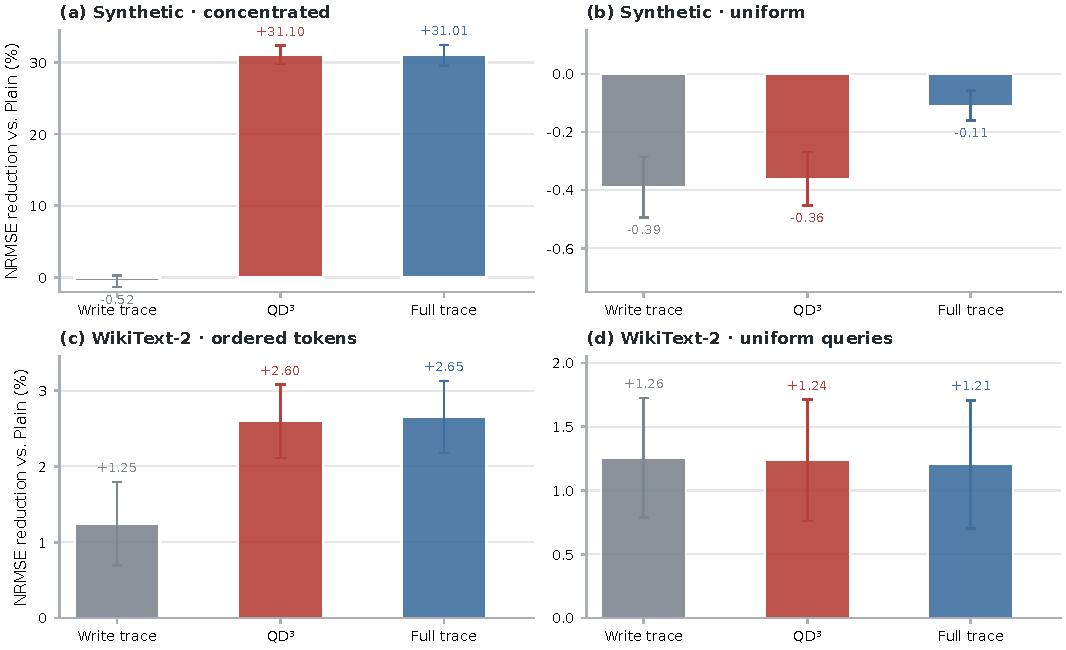
\includegraphics[width=0.96\linewidth]{figures/Fig2_main_results.pdf}
\caption{相对普通 Delta 的盲测 NRMSE 降幅，显示 16 个种子的均值和配对 95\% 置信区间，每个子图使用各自标注的纵轴尺度。在受控空间场上，查询轨迹改善集中查询条件下的回忆，而匹配的写入轨迹无改善；查询变为均匀后，两者差异消失。在 WikiText-2 上，连续留出查询使 \QDDD\ 获得 2.62\% 的降幅；均匀查询下，\QDDD\ 与写入轨迹几乎相同。NRMSE 越低越好。}
\label{fig:main-results-zh}
\end{figure}

\subsection{收益来源}

图\ref{fig:mechanism-zh}(a) 的查询偏斜扫描连续改变假设中的原因，而不是只比较两个端点。当 $\alpha=0$ 时，\QDDD\ 相对写入轨迹没有可测优势。随着读取需求更加集中，这一优势单调增长；当 $\alpha=1.25$ 时，在词元轮廓和导入图上分别达到 2.90\% 和 7.20\%。如果第二个状态确实测量了工作负载不匹配，就应观察到这种模式：只改变查询分布，而保持写入对象不变，查询历史的价值随之改变。

图\ref{fig:mechanism-zh}(b) 和表\ref{tab:ablation-zh} 检验轨迹表示方式。固定随机秩四子空间几乎无效，说明单纯增加相同数量的状态不足以产生收益。对角轨迹在需求与输入坐标对齐时有效，却无法处理旋转后的空间特征。最近一次查询能够捕获部分局部性，但在空间任务上始终弱于累积几何。秩一到秩四的学习查询轨迹在两个真实数据构造任务上基本恢复了完整轨迹的全部收益；空间场则需要 4 个方向才能取得最佳测试均值。更高秩并不必然更好，因为验证阶段需要为整个状态选择一组全局 $(\eta,\beta)$，有限数据流中的子空间估计也会变得更嘈杂。结果支持压缩工作负载统计量，但不意味着存在对所有任务通用的唯一秩。

\begin{figure}[t]
\centering
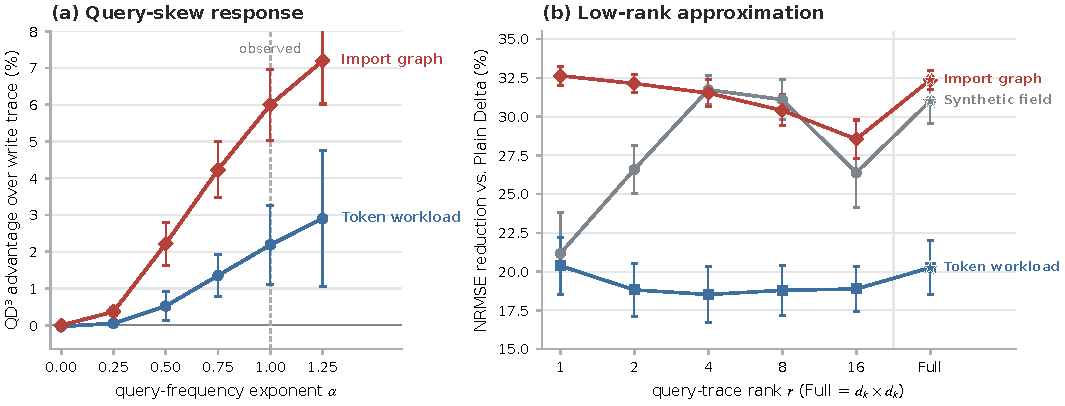
\includegraphics[width=0.96\linewidth]{figures/Fig3_mechanism_and_ablation.pdf}
\caption{盲测种子上的机制检验。(a) 随着查询频率指数增大，\QDDD\ 相对估计器与容量匹配的写入轨迹获得更多 NRMSE 降幅；均匀查询时该优势接近零。(b) 小型自适应查询子空间可以恢复完整在线二阶矩的结果；最佳秩取决于任务，并且只使用验证种子选择。}
\label{fig:mechanism-zh}
\end{figure}

\begin{table}[t]
\caption{消融结果，以相对普通 Delta 的 NRMSE 降幅百分比表示。“随机”使用固定随机秩四子空间；“最佳低秩”仅为解释而报告盲测均值最好的候选秩，表\ref{tab:main-zh} 中的所有主要秩均只根据验证数据选择。}
\label{tab:ablation-zh}
\centering
\small
\begin{tabular}{lrrrrr}
\toprule
工作负载 & 对角 & 最近查询 & 随机 & 最佳低秩 & 完整轨迹 \\
\midrule
集中空间场 & $-0.82$ & $16.09$ & $-0.64$ & $31.73$ ($r=4$) & $30.91$ \\
源代码词元轮廓 & $18.30$ & $20.12$ & $1.70$ & $20.53$ ($r=1$) & $20.40$ \\
模块导入图 & $27.50$ & $30.71$ & $3.00$ & $32.65$ ($r=1$) & $32.37$ \\
\bottomrule
\end{tabular}
\end{table}

\subsection{变化的需求}

移动热点实验在数据流进行到一半时改变查询中心，并在最终区域上评估。普通 Delta 的 NRMSE 为 $0.7528\pm0.0241$，写入轨迹为 $0.7630\pm0.0346$。\QDDD\ 达到 $0.5600\pm0.0390$，相对普通 Delta 降低 25.6\%。它还比稠密完整轨迹的 $0.5814\pm0.0484$ 低 $0.0214$ NRMSE，配对 95\% 置信区间为 $[-0.0329,-0.0100]$。低秩瓶颈和指数能量衰减共同偏向近期占主导的方向，因此在需求移动时具有优势。我们把这一结果解释为在线跟踪证据，而不是低秩结构一定优于完整矩的普遍保证。

\section{讨论}\label{sec:discussion-zh}

\subsection{设计解释}

写入轨迹已经排除了“任意自适应速率都有效”这一解释。实验支持的是预期信息流：读取估计需求，该估计为后续写入分配修正力度，值状态仍负责关联本身。式\eqref{eq:query-risk-zh} 指定记忆应服务的总体，式\eqref{eq:heat-identity-zh} 则只利用地址给出在线几何代理。该代理不是密度比估计器，也不替代加权线性解；其创新在于用 $O(d_kr)$ 状态实现满足因果性、可检查且能持续更新的读取感知分配。均匀控制补全了这一解释：当读取和写入包含的信息可互换时，两种匹配轨迹表现一致；当访问集中到键空间中的其他区域时，结果才会分离。

\subsection{应用价值与部署范围}

合适的部署对象具有三项可观测性质：关联持续到达但容量固定；读取发生在之后的某些写入之前；访问比被存储的总体更加集中。最贴近的场景是线性注意力或快速权重序列层，因为其循环矩阵已经是连续叠加，不存在可逐项淘汰的词元列表。其他自然场景包括长期智能体或检索记忆，其中重复请求能够暴露语义需求；以及机器人或传感器地图，其中反复访问的区域应在后续更新中获得更高精度。在这些场景中，访问摘要始终保持为 $O(d_kr)$，不会扩张成不断增长的日志。

部署前可以直接从容量压力和访问统计检查这些条件。一次性构建的存储没有因果读取信号，均匀访问也没有信息源特有的分配优势。因此，下一步不是扩大主张范围，而是把算子整合进分块训练内核，并测量下游语言、检索和具身记忆性能。

\section{结论}\label{sec:conclusion-zh}

查询双动态 Delta 把历史访问转化为未来存储的紧凑因果信号。低秩轨迹学习查询方向和能量，归一化且带上限的热度调节普通残差 Delta 写入，令 $\beta=0$ 则精确恢复基础规则。在受控与留出任务上，当需求集中时，查询信息能够改善回忆，并稳定优于估计器匹配的写入信息。由此得到的设计结论十分明确：对于持续更新的固定容量记忆，读取可以指导之后的写入分配，而无需保留不断增长的访问历史。

\section*{声明}

\noindent\textbf{利益冲突。}作者声明不存在与本文相关的财务或非财务利益冲突。

\noindent\textbf{经费。}本研究、论文写作与发表未获得财务资助。

\noindent\textbf{作者贡献。}Dian Yu 提出方法，设计并实施实验，分析结果并起草论文；Haoyu Yang 审阅并修改论文。两位作者均阅读并批准最终稿。

\noindent\textbf{伦理审批。}不适用。本研究使用公开文本和本地构建的软件结构统计，不涉及人类参与者。

\noindent\textbf{参与同意。}不适用。

\noindent\textbf{发表同意。}不适用。

\noindent\textbf{数据可用性。}WikiText-2 是由 Merity 等人引入的公开语料库\cite{merity2016wikitext}。本文报告实验实际使用的完整预处理数组包含在随稿复现包中。

\noindent\textbf{代码可用性。}全部记忆算子、验证与测试评估、统计分析和实现检查的源代码均包含在随稿材料中，并将在论文接收后存入公开仓库。

\bibliographystyle{unsrt}
\bibliography{references}

\end{document}
